\documentclass{beamer}
\usetheme{Madrid}
\useinnertheme{rounded}
\usecolortheme{whale}

\title{Next Reaction Method}
\subtitle{Efficient Stochastic Simulation of Chemical Systems}
\author{Lorenzo Beretta}
\date{29th July 2019}

%pacchetti scrittura
\usepackage{dsfont}
\usepackage{amsthm}
\usepackage{amsmath}
\usepackage{amssymb}
\usepackage{mathrsfs}
\usepackage{mathtools}
\usepackage{enumitem}
\usepackage{hyperref}
\usepackage{marginnote}
\usepackage{scalerel}
\usepackage{comment}
\usepackage[utf8]{inputenc}

%% miei %%
\usepackage{tkz-graph}
\usepackage{algorithm,algorithmic}
\usepackage{tikz}
\usepackage{color}
\usepackage{centernot}
\usepackage{esvect}

% tikz
\usetikzlibrary{positioning,chains,fit,shapes,calc}
\definecolor{myblue}{RGB}{80,80,160}
\definecolor{mygreen}{RGB}{80,160,80}

\begin{document}

\begin{frame}
  \maketitle
\end{frame}

\begin{frame}{Predictive Model Definition}
  To define a predictive model we need two steps:
  \begin{itemize}
  \item $\bullet$ Define a descriptive model of the phenomenon
    \begin{block}{Descriptive Model: Differential Equation}
      The Newton's law of motion:
      $$ \vv{F} = m \, \frac{\partial^2 \vv{x}}{\partial t^2} $$
    \end{block}    
  \item $\bullet$ Define a computational model to make predictions
    \begin{block}{Computational Model: Numerical Integration}
      \begin{figure}[h]
        \centering
        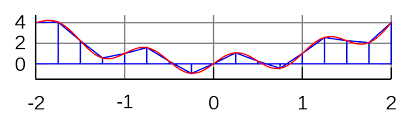
\includegraphics[scale=0.6]{num_int}
      \end{figure}
    \end{block}
  \end{itemize}
\end{frame}

\begin{frame}{Coupled Chemical System: Mathematical Description}
  \begin{columns}
    \begin{column}{.45 \textwidth}
     \begin{block}{Set of Elementary Reactions}
      \begin{equation*}
        \begin{gathered}
          A + B \rightarrow C \\
          B + C \rightarrow D \\
          D + E \rightarrow E + F \\
          F \rightarrow D + G \\
          E + G \rightarrow A   
        \end{gathered}
      \end{equation*}
    \end{block}
    \end{column}
    \begin{column}{.45 \textwidth}
      \begin{block}{Model Assumptions}
        \begin{itemize}
        \item $\bullet$ Many molecules: continuous and deterministic
        \item $\bullet$ Few molecules:\\ discrete and stochastic
        \end{itemize}
    \end{block}
    \end{column}
  \end{columns}
\end{frame}


\begin{frame}{Deterministic Framework}
  \begin{columns}
   \begin{column}{.45 \textwidth}
     \begin{block}{Set of Elementary Reactions}
      \begin{equation*}
        \begin{gathered}
          A + B \rightarrow C \\
          B + C \rightarrow D \\
          D + E \rightarrow E + F \\
          F \rightarrow D + G \\
          E + G \rightarrow A   
        \end{gathered}
      \end{equation*}
    \end{block}
    \end{column}
     \begin{column}{.45 \textwidth}
      \begin{block}{Computation}
        \begin{equation*}
          \begin{gathered}
            \frac{\partial [A]}{\partial t} = f_A\left([A], \dots [G]\right) \\
            \frac{\partial [B]}{\partial t} = f_B\left([A], \dots [G]\right) 
            &\vdots\\
            \frac{\partial [G]}{\partial t} = f_G\left([A], \dots [G]\right) \\
      \end{gathered}
      \end{equation*}
      \end{block}
    \end{column}
  \end{columns}
\end{frame}

\begin{frame}{Stochastic Framework}
  \begin{columns}
    \begin{column}{.45 \textwidth}
     \begin{block}{Set of Elementary Reactions}
      \begin{equation*}
        \begin{gathered}
          R_1 + R^\prime_2 \xrightarrow{k_1} P_1 \\
          R_2 + R^\prime_2 \xrightarrow{k_2} P_2 \\
          R_3 + R_3^\prime \xrightarrow{k_3} P_3 + P_3^\prime 
         \end{gathered}
      \end{equation*}
    \end{block}
    \end{column} 
    \begin{column}{.45 \textwidth}
      \begin{block}{Propensity $k_i$}
        The probability that $i$-th reaction occurs
         in  $[0, dt]$ is
         $$k_i dt + o(dt)$$
         fixing molecules IDs a priori.
       \end{block}
    \end{column}
  \end{columns}
  \begin{block}{Reaction Rate $a_i$}
         The probability that $i$-th reaction occurs
         in  $[0, dt]$ is
         $$a_i dt + o(dt)$$
         with
         $$ a_i = k_i \cdot \#R_1 \codt \dots \#R_n$$
  \end{block}
\end{frame}

\begin{frame}{Stochastic Framework}
  \begin{block}{Model Assumptions}
    \begin{itemize}
    \item $\bullet$ Molecules in solution $\implies$ No position $\implies$ States are multisets

      \begin{center}
        \begin{minipage}{.7 \textwidth}
          \begin{block}{State}
            $$ S = \left\{ \#M_1, \, \dots \#M_m \right\} $$
          \end{block}
        \end{minipage}
      \end{center}
      
      \item $\bullet$ Propensities are constant 

        \begin{center}
          \begin{minipage}{.7 \textwidth}
            \begin{block}{State}
              If $a_1$ reaction turns $S$ into $S^\pirme$, then for each $t > 0$
              $$ \mathbb{P}\left(S^\prime, t + dt \,  \left | \, S, t\right\right) = a_1dt + o(dt) $$
            \end{block}
          \end{minipage}
        \end{center}
  
      \end{itemize}
  \end{block}
\end{frame}

\begin{frame}{Master Equation}
  The model is finite state CTMC exactly
  \begin{itemize}
  \item $\bullet$ One variable for each state
  \item $\bullet$ transition probabilities $\longrightarrow$ differential equations 
  \item $\bullet$ Exponential number of states
  \end{itemize}
\end{frame}

\begin{frame}{SNIPPETS}
  \begin{center}
    \begin{minipage}{.7 \textwidth}
      \begin{block}{Teorema}
        In quasi ogni torneo ogni vertice è un King.
      \end{block}
    \end{minipage}
  \end{center}
  \begin{columns}
  \begin{column}{.45 \textwidth}
    \begin{block}{Set of Elementary Reactions}
      \begin{equation*}
        \begin{gathered}
          R_1 + R^\prime_2 \xrightarrow{k_1} P_1 \\
          R_2 + R^\prime_2 \xrightarrow{k_2} P_2 \\
          R_3 + R_3^\prime \xrightarrow{k_3} P_3 + P_3^\prime 
        \end{gathered}
      \end{equation*}
    \end{block}
  \end{column} 
  \begin{column}{.45 \textwidth}
    \begin{block}{Propensity $k_i$}
      The probability that $i$-th reaction occurs
      in  $[0, dt]$ is
      $$k_i dt + o(dt)$$
      fixing molecules IDs a priori.
    \end{block}
  \end{column}
\end{columns}
\end{frame}

\begin{frame}
  \begin{center}
  \Huge{Thank you for your attention.}
  \Huge{Questions?}
  \end{center}

\end{frame}

\end{document}

%%% Local Variables:
%%% mode: latex
%%% TeX-master: t
%%% End:
